
\documentclass[border=10pt]{standalone}
\usepackage[table]{xcolor}
\usepackage{amsmath,amssymb,amsfonts,mathtools,bm}
\usepackage{booktabs,array}
\usepackage{tikz}
\usetikzlibrary{arrows.meta,positioning,calc,backgrounds,fit,shapes.geometric,decorations.pathreplacing}
\usepackage{pgfplots}
\pgfplotsset{compat=1.18}
\definecolor{sbnavy}{HTML}{1A2A4F}
\definecolor{sbteal}{HTML}{1C7293}
\definecolor{sbaccent}{HTML}{B5651D}
\definecolor{sbgrey}{HTML}{8A94A6}
\definecolor{sblight}{HTML}{EAF1F5}
\newcommand{\cmark}{\textcolor{sbteal}{\ensuremath{\boldsymbol{\checkmark}}}}
\newcommand{\xmark}{\textcolor{sbgrey}{\ensuremath{\boldsymbol{\times}}}}
\newcommand{\eqcol}{\color{sbnavy}}
\begin{document}
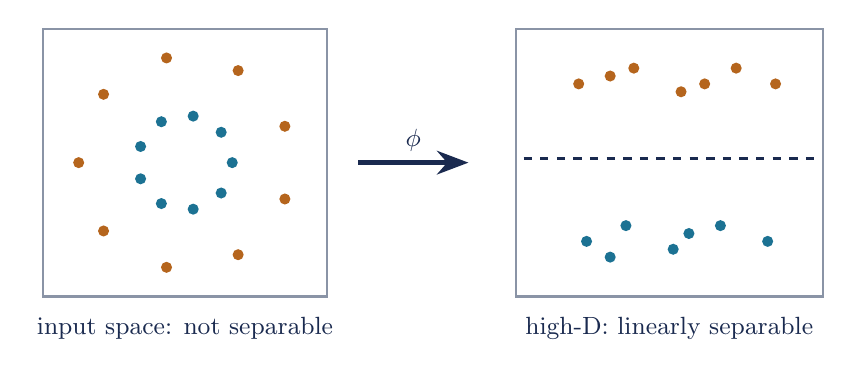
\begin{tikzpicture}[font=\sffamily]
  % left: 2D not separable (two interleaved rings)
  \begin{scope}
    \draw[sbgrey,line width=0.8pt] (-0.2,-0.2) rectangle (3.4,3.2);
    \foreach \a in {0,40,...,320}{ \fill[sbteal] ($(1.6,1.5)+(\a:0.6)$) circle (2pt);}
    \foreach \a in {20,60,...,340}{ \fill[sbaccent] ($(1.6,1.5)+(\a:1.35)$) circle (2pt);}
    \node[font=\small,sbnavy] at (1.6,-0.6) {input space: not separable};
  \end{scope}
  \draw[-{Stealth[length=4mm]},line width=1.6pt,sbnavy] (3.8,1.5) -- (5.2,1.5) node[midway,above,font=\small]{$\phi$};
  % right: lifted, separable by a plane
  \begin{scope}[shift={(6.0,0)}]
    \draw[sbgrey,line width=0.8pt] (-0.2,-0.2) rectangle (3.7,3.2);
    \fill[sbteal] (0.7,0.5) circle (2pt) (1.2,0.7) circle (2pt) (1.8,0.4) circle (2pt) (2.4,0.7) circle (2pt) (3.0,0.5) circle (2pt) (1.0,0.3) circle (2pt) (2.0,0.6) circle (2pt);
    \fill[sbaccent] (0.6,2.5) circle (2pt) (1.3,2.7) circle (2pt) (1.9,2.4) circle (2pt) (2.6,2.7) circle (2pt) (3.1,2.5) circle (2pt) (1.0,2.6) circle (2pt) (2.2,2.5) circle (2pt);
    \draw[sbnavy,dashed,line width=1.2pt] (-0.1,1.55) -- (3.6,1.55);
    \node[font=\small,sbnavy] at (1.75,-0.6) {high-D: linearly separable};
  \end{scope}
\end{tikzpicture}
\end{document}